% This is samplepaper.tex, a sample chapter demonstrating the
% LLNCS macro package for Springer Computer Science proceedings;
% Version 2.20 of 2017/10/04
%
\documentclass[runningheads]{llncs}
%
\usepackage{graphicx}
\usepackage[utf8]{inputenc}
\usepackage[T1]{fontenc}
\usepackage{hyperref}
\usepackage{amsfonts}
\usepackage[section]{placeins}
\hypersetup{
    colorlinks=true,
    linkcolor=black,
    filecolor=magenta,      
    urlcolor=red,
}
\usepackage{amsmath}
\usepackage{listings}
\usepackage{float}
\usepackage{color}
\usepackage{minitoc}
\usepackage[french,english]{babel}
\definecolor{codegreen}{rgb}{0,0.6,0}
\definecolor{codegray}{rgb}{0.5,0.5,0.5}
\definecolor{codepurple}{rgb}{0.58,0,0.82}
\definecolor{backcolour}{rgb}{0.95,0.95,0.92}
 
\lstdefinestyle{mystyle}{
    backgroundcolor=\color{backcolour},   
    commentstyle=\color{codegreen},
    keywordstyle=\color{magenta},
    numberstyle=\tiny\color{codegray},
    stringstyle=\color{codepurple},
    basicstyle=\footnotesize,
    breakatwhitespace=false,         
    breaklines=true,                 
    captionpos=b,                    
    keepspaces=true,                 
    numbers=left,                    
    numbersep=5pt,                  
    showspaces=false,                
    showstringspaces=false,
    showtabs=false,                  
    tabsize=2
}
 
\lstset{style=mystyle}

\begin{document}
\selectlanguage{french}


\title{Factorisation matricielle non-n\'egative et classification d'images}

\author{MOHAMED BEN HAMDOUNE\inst{1} et YANNIS TANNIER\inst{1}}

\authorrunning{M. Ben Hamdoune et al.}

\markboth{M. Ben Hamdoune, Y. Tannier}{Factorisation matricielle non-n\'egative et classification d'images}

\institute{Universit\'e Paris-Descartes, 12 Rue de l'\'Ecole de M\'edecine, 75006 Paris, France,
\email{mohamed.ben\_hamdoune@etu.parisdescartes.fr}\\ 
\\
\email{yannis.tannier@etu.parisdescartes.fr}\\
\url{https://www.univ-paris5.fr/}}

\maketitle

\begin{abstract}
La classification automatique ou $clustering$ consiste \`a partionner un ensemble d'objets (instances) d\'ecrit par un ensemble de variables en groupes (classes) homog\`enes. Avec l'av\`enement du $Big Data$ et de la science des donn\'ees, le clustering est devenu une t\^ache tr\`es importante dans divers domaines dont l'imagerie. Les images sont des donn\'ees tr\`es r\'epandues notamment sur le web et les r\'eseaux sociaux (Instagram, Pinterest, Flickr, Google,etc...).Le but sera de proposer un syst\'eme de classification pour des images provenant de divers bases de donn\'ees (photos, peintures, bandes dessin\'es, etc). La factorisation matricielle non-n\'egative permet d'approximer une matrice de donn\'ees positive par le produit de deux matrices de dimensions inf\'erieures et positives. Par sa simplicit\'e, cette m\'ethode est devenue populaire et est utilis\'ee \`a la fois dans la r\'eduction de la dimension et \'egalement dans la classification automatique (clustering) en un nombre de classes $k$ fix\'e par l'utilisateur. 
\keywords{Apprentissage Non Supervis\'e, Spherical K-means, K-means, R, NMF, Python, Scikit-Learn, Nimfa, People-Art Dataset}
\end{abstract}

\setcounter{tocdepth}{3}
\setcounter{secnumdepth}{3}
\tableofcontents
\newpage

\section*{Remerciements}
Nous souhaitons adresser nos remerciements aux personnes qui nous ont aidé dans la réalisation de ce rapport. \\
En premier lieu, nous remercions M. Nadif et M. Labiad qui nous ont permis d'accéder à leur publications.\\
Nous remercions aussi M. Salem, notre responsable du master, pour son modèle de rédaction ainsi que ces informations durant cette année scolaire.\\
Enfin, nous souhaitions particulièrement remercier M.Febressy pour sa disponibilité tout au long de ce semestre ainsi que sa précieuse aide à la relecture et à la correction de notre rapport.

\newpage

\section{Introduction}
\subsection{Contexte et motivations}

Dans le cadre de notre cursus scolaire, nous sommes amenés à réaliser un TER \textbf{(Travail d'étude et de recherches)}. Notre sujet est intitulé : \textbf{"Factorisation matricielle non-négative et classification d'images"}. Au cours de ce semestre nous avons étudié la NMF (\textbf{Non-Negative Matrix Factorization}) et aussi sa particularité à faire de la classification automatique (\textit{clustering}) dans certains cas comme cela sera décrit dans ce rapport.
La NMF est un sujet très intéressant car elle couvre de nombreux domaines :  imagerie, reconnaissance de formes, fouille de textes. La recommandation est également un domaine o\`u la NMF excelle et a permis de nombreuses avancées.
Enfin, la NMF peut être une technique très puissante de réduction de dimension adaptée aux matrices creuses contenant des données positives, par exemple des occurrences ou dénombrements de mots.

\subsection{Contribution et organisation du rapport}

Le déroulement de ce \textbf{TER} suit finalement une logique qui est propre aux systèmes lors d'une modélisation de classification automatique.
Tout d'abord comme écrit dans la première consigne, nous avons réalisé la matrice (Section \ref{constmat}), c'est-à-dire converti les images de départ disponibles sur \textit{Github} [\href{https://github.com/BathVisArtData/PeopleArt/tree/master/JPEGImages}{ici}] dans un format qui permet d'être applicable dans une NMF. Les filtres (Section \ref{filtre}) disponibles les plus courants sont binaires, niveaux de gris, RGB. Pour ce TER, nous avons décidé d'appliquer un filtre greyscale.
De plus nous discuterons sur la normalisation (Section \ref{norm}) de cette matrice pour ensuite passer à la section suivante sur les méthodes d'analyse.
Nous introduirons la notion de NMF (Section \ref{nmf}) comme méthode de factorisation matricielle non-négative et les deux méthodes de partitionnement utilisées que sont \textit{K-means} et \textit{Spherical K-means} permettant de faire du clustering avec la NMF.
\`A partir de tout cela, nous réaliserons une étude comparative (Section \ref{comparative}) avec plusieurs combinaisons d'initialisation pour réaliser la NMF suivant un intervalle donné par les résultats de \textit{K-means} et \textit{Spherical K-means}.
Finalement, nous conclurons (Section \ref{conclusion}) sur ce projet avec les idées que nous avions et que nous n'avons pas pu réaliser, ainsi que notre avis sur ce sujet de TER.

\section{Construction de la matrice num\'erique}

\subsection{Construction de la matrice}
\label{constmat}

Le jeu de données qui nous a été donné à pour thématique \textit{l'art} et plus précisément une collection d'images couvrant une grande variété de styles artistiques. Cette collection \cite{westlake2016detecting} regroupe en tout 4778 images regroupées dans 43 dossiers (catégories).
Ces images ont été rassemblé dans le but de faire de la \textit{cross-depiction} (La représentation croisée est la reconnaissance et la synthèse des objets qu'ils soient photographiés, peints, dessinés, etc. C'est un problème important mais sous-étudié. Le but étant de reproduire artificiellement la capacité humaine de reconnaître et de représenter des objets).
Les images sont diverses et variées et ils sont sous \textit{"copyright"}. Elles sont essentiellement mises à disposition pour l'exploration de données dans un cadre de recherche non-commercial.
Afin d'avoir une uniformisation entre les images pour effectuer l'analyse, nous avons d'abord redimensionné la taille de chaque image en 25x25.
Pour cela nous avons utilisé \textbf{Pillow}, une librairie Python \cite{python} qui permet de faire de la manipulation d'image. Toutes les images redimensionnées ont été enregistrées dans un dossier "resized" afin de pouvoir être réutilisées plus tard. Enfin le label (la catégorie de l'image) a également été récupéré.

\begin{lstlisting}[language=Python]
images = glob.glob("PeopleArt/JPEGImages/*/*")
i = 1
for image in images:
    label = image.split("/")[2].lower()
    with open(image, 'r+b') as f:
        img = Image.open(f)
        img = resizeimage.resize_cover(img, [25, 25])
        img.save("PeopleArt/resized/"+label+"_"+str(i)+'.jpg', img.format)
    i += 1

\end{lstlisting}

\subsection{Les filtres num\'eriques}
\label{filtre}

Une fois les images redimensionnées, nous avons appliqué diffèrents filtres.
Pour cela, nous avons utilisé la librairie \textbf{Pillow} en \textit{Python} qui propose plusieurs filtres : \\ - Le filtre niveau gris (\textit{"greyscale"}) qui retourne des valeurs $x \in \mathopen[0,255\mathclose]$. \\ - Le filtre binaire ("\textit{binarisation}") des images  retournant des valeurs qui sont soit 0 ou 1 suivant un seuil \textit{"threshold"}. \\ - Le filtre \textit{RGB} (Red-Green-Blue), qui retourne une matrice en 3 dimensions représentant chaque couleur.
Dans le cadre de ce rapport, nous avons choisi le filtre greyscale par soucis de temps de calcul assez conséquent.\\ \\
Pour créer notre matrice, nous avons donc converti chaque image en greyscale. Pillow nous retourne ainsi une matrice 25x25 comprenant des valeurs entre 0 et 255. Nous avons ensuite transformé cette matrice en vecteur de taille 625 et nous avons concaténé tout les vecteurs d'images afin de former notre matrice. La matrice finale comprend ainsi 4778 lignes et 625 colonnes. 

\begin{lstlisting}[language=Python]
images = shuffle(glob.glob(folder+"*"))
labels = np.array([])
X_data = np.array([])

for image in images:    
    labels = np.append(labels,image.split("/")[3].split("_")[0].lower())    
    image = Image.open(image).convert('L')
    arr = np.array(image)
    arr = arr.reshape(1,size*size)    
    X_data = np.concatenate((X_data, arr), axis = 0)
np.savetxt('gs.csv', X_data, fmt = '%3d', delimiter = ',')
\end{lstlisting}


\subsection{Normalisation}
\label{norm}

Une fois notre matrice crée, nous avons appliqué une normalisation en ligne.
Cette normalisation consiste à appliquer une normalisation $L_2$ afin de mettre le vecteur à l'échelle et ainsi obtenir un vecteur unitaire. Un vecteur unitaire correspond à un vecteur dont la norme est égale à 1. \\
Ainsi, étant donnée notre matrice $X$, ou les lignes correspondent aux observations et les colonnes aux caractéristiques, nous avons divisé chaque vecteur $x \in X$ par la norme $L_2$ du vecteur :

$$L_2 =  ||x||_{2} = \sqrt{\sum_{i} x_{i}^2 }.$$
\linebreak
Cela peut être fait très facilement en Python grâce à la librairie \textbf{Scikit-Learn} \cite{scikit-learn} :

\begin{lstlisting}[language=Python]
from sklearn import preprocessing
X_normalized = preprocessing.normalize(datas, norm = 'l2')
\end{lstlisting}

\section{Clustering}

Le partitionnement de données (ou clustering) est une des méthodes d'analyse des données qui vise à diviser un ensemble de données en différents "groupes" homogènes, c'est-à-dire que les données de chaque sous-ensemble partagent des caractéristiques communes, qui correspondent le plus souvent à des critères de proximité. Dans ce rapport nous verrons deux méthodes de clustering que nous avons utilisé : K-means et Spherical K-means.

\subsection{K-means et Spherical K-means}

\textbf{K-means} est une méthode de partitionnement de données qui, à partir d'un ensemble de points, va pouvoir déterminer pour un nombre de classes fixé une répartition des points qui minimise un critère appelé \textit{inertie} ou variance \textit{intra-classe}. \\
Plus formellement étant donnée $k$,  nous allons donc chercher à répartir les points $x_{1}, x_{2}, .., x_{n}$ en $k$ groupes $C_{1},C_{2},…,C_{K}$ de telle sorte que :
$$ \sum_{k=1}^K \frac {1}{|C_{k}|}  \sum_{x\in C_{k}} || x - ( \frac{1}{|C_{k}|} \sum_{x\in C_{k}} x) ||^2 $$ soit le plus minimale.
\\ \\
\textbf{Spherical K-means} contrairement à K-means qui cherche à minimiser une distance euclidienne, on va plutôt définir le centre de chaque groupe de sorte à uniformiser et minimiser l'angle entre les composants.

\subsection{Déterminer le nombre de cluster $k$}

Comme nous l'avons vu précédemment, il est essentiel d'indiquer le bon nombre de cluster à K-means et Spherical K-means. Cependant déterminer le bon nombre de cluster est une tâche qui peut s'avérer très compliquée. 
Pour cela nous avons choisi 2 critères afin d'évaluer la qualité du partitionnement : la méthode \textbf{du Coude} et le coefficient de \textbf{Silhouette} (Des packages comme \textit{"facto extra"} et \textit{"Nbclust"} facilitent la possibilité d'effectuer un graphique sur les méthodes permettant d'avoir une idée sur le nombre de classe avec R \cite{rproject}).
\\ \\
- La méthode du Coude : L'idée derrière cette méthode est d'exécuter K-Means sur l'ensemble des données pour un nombre de cluster de valeurs $k$ (par exemple $k$ = 1 à 10) et de calculer pour chaque rang $k$ la somme des erreurs au carré ($SSE$). Ainsi on peut choisir un nombre de cluster $k$ de telle sorte que l'ajout d'un autre cluster ne donne pas une meilleure modélisation des données. \\
Cette méthode s'appelle aussi la méthode du \textit{"coude"} car si on affiche les informations sur un graphe, nous pouvons choisir le rang $k$ au niveau où la courbe forme un \textit{"coude"}. \\ \\
- Le coefficient de Silhouette : Cette méthode est une mesure de la similitude entre un objet et son propre cluster (cohésion) par rapport aux autres clusters (séparations). Autrement dit, le coefficient de silhouette $s(x)$ permet d'évaluer, pour un point $x$ donné, si ce point appartient au "bon" cluster : est-il proche des points du cluster auquel il appartient ? Est-il loin des autres points ? \\ 
La valeur de la silhouette est compris entre -1 et 1 où plus la valeur est proche de 1 et plus l'assignation de $x$ à son cluster est satisfaisante.
\\

\subsection{Analyse et résultats}

Afin de déterminer un intervalle de rang, nous avons appliqué la formule : $$R = \frac{m*n}{m+n}$$ où $m$ correspond au nombre de lignes de notre matrice et $n$ le nombre de colonne. 

\begin{figure}[H]
\centering
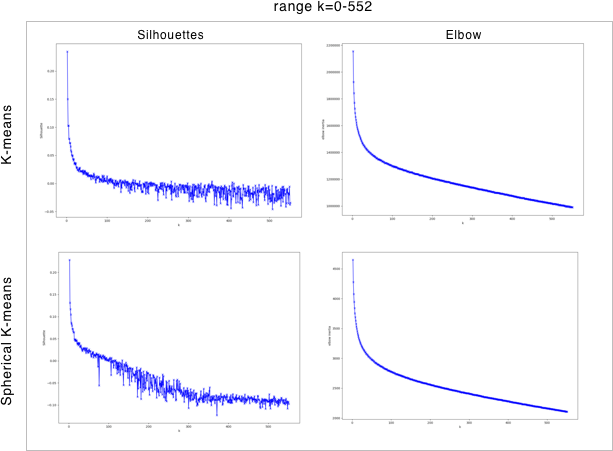
\includegraphics[width=1\textwidth]{552.png}
\caption{Mesures de K-means et Spherical K-means sur les rangs de 0 à 552.}
  \label{fig:552}
\end{figure}

Les résultats en Figure 1 nous montrent qu'une analyse précise de la silhouette et de la méthode du coude est assez compliqué avec un intervalle de rang aussi grand. Cependant nous pouvons déjà voir qu'entre 20 et 70, les graphiques semblent intéressant pour K-means et Spherical K-means. De plus on sait également que nos images sont classées en 43 catégories (dossier), cela nous donne une première estimation du rang que l'on pourrait trouver. 
Nous nous y sommes donc intéressées et avons refait les analyses avec cet nouvel intervalle.


\begin{figure}[H]
\centering
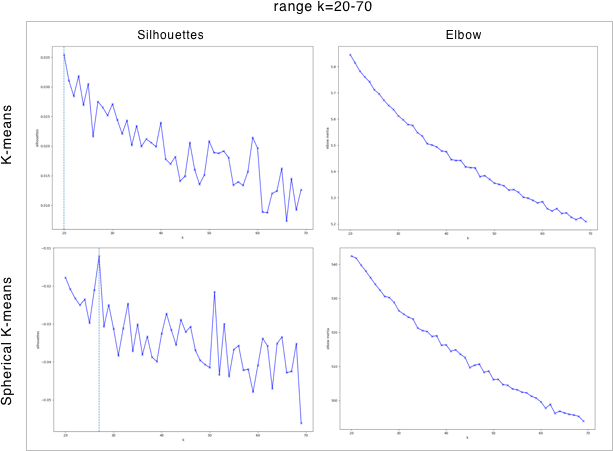
\includegraphics[width=1\textwidth]{70.png}
\caption{Mesures de K-Means et Spherical K-means sur les rangs de 0 à 552.}
  \label{fig:70}
\end{figure}

Ainsi, nous pouvons voir que d'après la Figure 2, la silhouette pour K-means semble meilleur pour les rangs 20, 23, 40, 59 et 27, 33, 41, 51 pour Spherical K-Means. Toutefois ces résultats sont à nuancer car la valeur la plus haute obtenue pour la silhouette est de 0.036, ce qui est très faible et nous donne une première indication quant à la qualité de partition.
Après avoir déterminé les rangs pour K-means et Spherical K-means, nous avons voulu comparer les résultats en calculant L'ARI et la NMI pour chacune des partitions obtenues avec la partition original, correspondant à la partition des catégories GitHub. En effet, ces catégories nous donnent une information sur un potentiel regroupement des images, ainsi nous avons voulu voir si ce regroupement correspond aux données.

\begin{figure}[H]
\centering
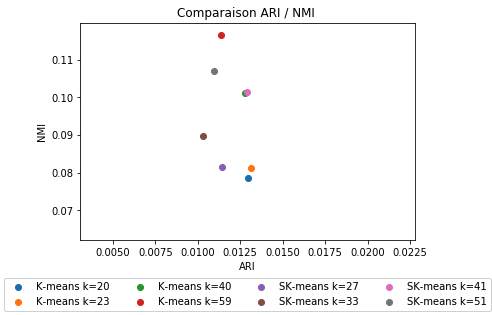
\includegraphics[width=1\textwidth]{clustering-comparaison.png}
\caption{Comparaison ARI/NMI sur les différents rangs.}
  \label{fig:clust-comp}
\end{figure}

Les résultats en Figure 3 nous montrent que les méthodes et les rangs se valent plus ou moins tous. Les résultats tournent autour de 0.08 et 0.012 pour la NMI et 0.01 et 0.15 pour l'ARI. Ces résultats sont faibles et vont dans le sens des résultats obtenus avec la silhouette.

Nous avons voulu aller plus loin en gardant cette information à priori sur le nombre de classe. Ainsi nous avons voulu tester les résultats obtenus avec les différentes méthodes et initialisation de la NMF avec $k = 43$. Nous avons calculé l'ARI/NMI et comparer avec la partition original (GitHub).

\begin{figure}[H]
\centering
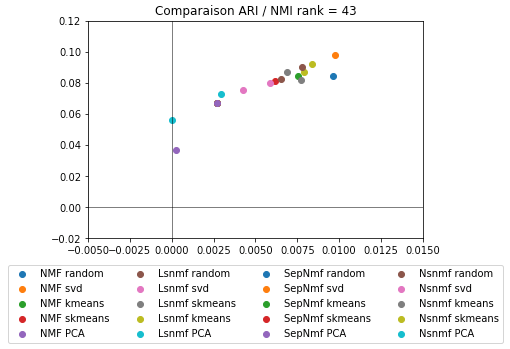
\includegraphics[width=0.8\textwidth]{ari_nmi_rank43.png}
\caption{Récapitulatif de l'ARI/NMI pour le rang 43.}
  \label{fig:k_sk-means43}
\end{figure}

Sans surprise les résultats sont très faible, confirmant ce que l'on a vu plus haut. Cependant nous pouvons voir que SepNmf avec une initialisation SVD et SepNmf avec une initialisation aléatoire s'en sortent le mieux, SepNmf étant une méthode de NMF particulièrement bien adapté pour les pixels. 

\begin{figure}[H]
\centering
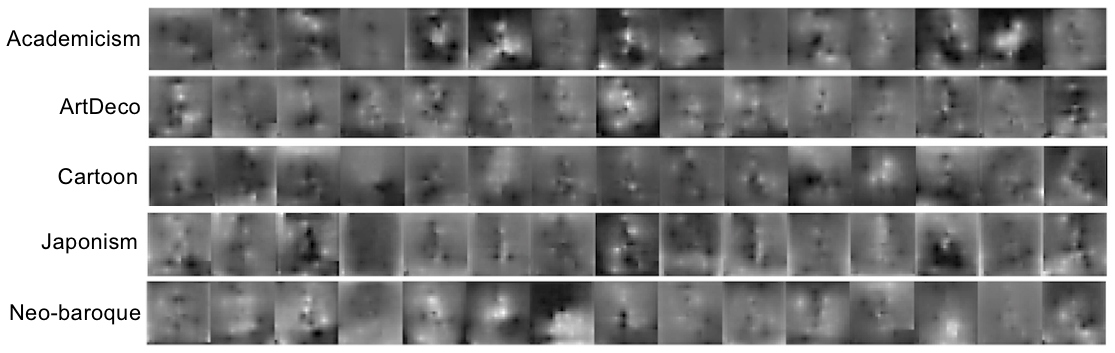
\includegraphics[width=0.8\textwidth]{recomposition.png}
\caption{Récapitulatif sur la recomposition des images.}
  \label{fig:recomposition}
\end{figure}

\par\bigskip 
\noindent

Enfin, la visualisation d'un échantillon d'image par catégorie nous montre bien que la NMF a du mal à extraire des caractéristiques spécifiques pour chaque classe.

Afin de renforcer nos résultats obtenus, nous avons par la suite utilisé une méthode de classification supervisé, la SVM, avec les matrices des images en features et la catégorie des images en labels.
\newpage


\begin{lstlisting}[language=Python]
from sklearn import svm
from sklearn.model_selection import cross_val_score

clf = svm.SVC()
scores = cross_val_score(clf, datas, labels, cv=10)

print("Accuracy: %0.2f (+/- %0.2f)" % (scores.mean(), scores.std() * 2))
# Accuracy: 0.05 (+/- 0.02) 
\end{lstlisting}


Nous obtenons une accuracy de 5\% via une validation croisée.

Ce dernier résultat nous pousse à conclure que la catégorisation originale est trop dispersée et qu'il n'existe sans doute pas de pattern permettant de différencier ces catégories.
Nous laissons donc tomber cette catégorisation et nous allons essayer de trouver la meilleure partition sur ce jeu de donnée sans considérer la catégorisation originale répartie sur les 43 dossiers.

C'est pour cette raison que nous avons calculé l'ARI et la NMI en croisant toutes les partitions obtenues, c'est-à-dire pour les rang 20, 23, 40, 59 pour K-means et 27, 33, 41, 51 pour Spherical K-means. Pour cela, nous avons créé un dendrogramme pour savoir qu'elles étaient les partitions les plus proches.

Enfin, on peut voir que pour K-means, les partitions 20, 23 et 40 sont relativement proche. Nous choisissons donc de garder uniquement la partition 20 et 59.
Pour Spherical K-Means, toutes les partitions se valent, nous gardons donc que la partition 27.


\begin{figure}[H]
\centering
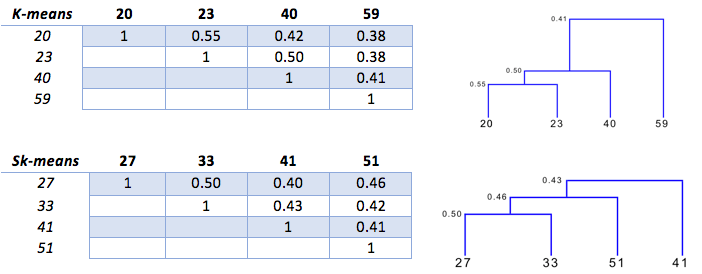
\includegraphics[width=1\textwidth]{ari_nmi.png}
\caption{Récapitulatif pour K-Means et Spherical K-Means avec leur arbre hiérarchique.}
  \label{fig:k_sk-means}
\end{figure}


\section{La factorisation matricelle non-négative}
\subsection{Présentation de la NMF}
\label{nmf}

Cette section donne une d\'efinition formelle des probl\`emes de factorisation matricielle non-n\'egative \cite{Gaujoux2010} et d\'efinit les notations utilis\'ees dans le cadre de ce TER.

Soit $X$ une matrice non-n\'egative $n \times p$, (i.e avec $x_{ij} \geq 0$,
telle que $X \geq 0$), et $r > 0$ un entier positif. 
La factorisation matricielle non-n\'egative consiste \`a trouver une approximation

\begin{equation}
X \approx W H\ , \label{NMFstd}
\end{equation} o\`u $W, H$ sont $n\times r$ et $r \times p$ matrices non-n\'egativs respectivement.

En pratique, le rang de factorisation $r$ est souvent choisi de telle sorte que $r \ll \min(n, p)$. 
L'objectif derrière ce choix est de r\'esumer et diviser l'information contenue dans $X$ en facteurs $r$: les colonnes de $W$.

Selon le domaine d'application, ces facteurs ont des noms diff\'erents: images de base, m\'etag\`enes, signaux source. Dans ce rapport, nous utilisons de mani\`ere \'equivalente et alternative les termes \emph{matrice des bases} pour faire r\'ef\'erence à la matrice $W$, et \emph{matrice de coefficients} pour se r\'ef\'erer à la matrice $H$.
La principale approche du \textbf{NMF} \cite{Gillis2014} consiste \`a estimer les matrices $W$ et $H$ comme un minimum local:
\begin{equation}
\min_{W, H \geq 0}\ \underbrace{[D(X, WH) + R(W, H)]}_{=F(W,H)} \label{nmf_min}
\end{equation}
o\`u

\begin{itemize}
\item $D$ est une fonction de perte qui mesure la qualit\'e de l'approximation.
Les fonctions de perte communes sont bas\'ees soit sur la distance de Frobenius
$$D: A,B\mapsto \frac{Tr(AB^t)}{2} = \frac{1}{2} \sum_{ij} (a_{ij} - b_{ij})^2,$$
ou la divergence Kullback-Leibler.
$$D: A,B\mapsto KL(A||B) = \sum_{i,j} a_{ij} \log \frac{a_{ij}}{b_{ij}} - a_{ij} + b_{ij}.$$
\item $ R $ est une fonction de r\'egularisation facultative, d\'efinie pour appliquer
les propri\'et\'es sur les matrices $W$ et $H$, telles que la \textit{$smoothness$} ou la \textit{$\text{sparsit\'e}$} \cite{Boutsidis2007}.
\end{itemize}

Un param\'etre critique dans la NMF est le rang de la factorisation $r$.
Il d\'efinit le nombre de variables utilis\'es pour approcher la matrice cible.
\'Etant donn\'e une m\'ethode NMF et la matrice cible, une façon courante de d\'ecider de $r $ est d'essayer diff\'erentes valeurs, de calculer une mesure de qualit\'e des r\'esultats et de choisir la meilleure valeur en fonction de ces critères de qualit\'e.

\subsection{Différentes méthodes de NMF}

Il existe plusieurs algorithmes permettant de réaliser une NMF (une librairie en Python du nom de Nimfa \cite{Zitnik2012} implémente plusieurs modèles de la NMF avec plusieurs algortihmes et plusieurs possibilités d'initialisation), généralement ces algorithmes fonctionnent de manière itérative, en construisant une séquence de matrice $(W, H)$ qui va tenter de réduire à chaque itération une \textit{fonction coût}. Il existe également des variantes de la fonction et d'autres techniques d'optimisation tel que la descente de gradient permettant de calculer et mettre à jour plus efficacement $H$ et $W$. \\
Dans la suite de ce rapport, nous expliquerons les diverses méthodes que nous avons utilisé : \\

 - \textbf{Brunet} : La première méthode utilisée est l'algorithme de brunet \cite{Brunet2004}, correspondant à la méthode Standard de NMF, basée sur la divergence de Kullback-Leibler. Cette méthode multiplicative est une amélioration de l'algorithme initialement proposé par Lee \cite{Lee2001} et permettant de réduire le \textit{numerical underflow}. \\

\begin{figure}[H]
\centering
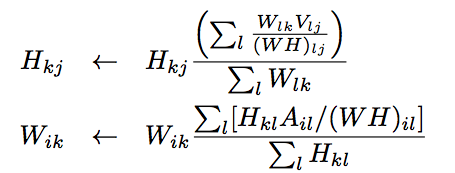
\includegraphics[width=0.5\textwidth]{brunet.png}
\label{fig:brunet}
\end{figure}

 - \textbf{Lsnmf} : Méthode de factorisation de la matrice des moindres carrés non-négatif utilisant une méthode de gradient (optimisation contrainte) pour chaque sous-problème. 
 Cette méthode proposée par Lin en 2007 \cite{Lin2007} a l'avantage de converger beaucoup plus rapidement que les approches courantes de mise à jour multiplicatives. \\

 - \textbf{Nsmf} : Nonsmooth Non negative Matrix Factorisation. Cette méthode proposée par Montano en 2006 est une version modifiée de la méthode de Lee permettant d'avoir de meilleur résultat dans le cas de matrice dite "\textit{sparse}" \cite{Boutsidis2007}. \\

 - \textbf{SepNmf} : Separable Nonnegative Matrix Factorization. Cette méthode a été proposée initialement par Donoho et Stodden en 2003 puis améliorée par Arora en 2012. La Sepnmf est particulièrement adaptée pour l'imagerie hyper-spectrale et l'analyse de document. \\

\section{Méthodes d'initialisation de la NMF}

\subsection{Aléatoire}
La plupart des fonctions coûts de la NMF ne sont pas convexes et sont donc sensibles à l'initialisation des matrices de facteurs $W$ et $H$ comme expliqué par N. Gillis \cite{Gillis2014}. Une bonne stratégie d'initialisation peut considérablement atténuer le problème de convergence des algorithmes NMF. Ici, le terme \textit{"bon"} se réfère à la stratégie d'initialisation qui conduit à une réduction rapide de l'erreur pour la fonction coût avec une vitesse de convergence rapide. Dans la littérature, l'initialisation aléatoire a été couramment utilisée, par exemple dans le travail de Lee et Seung \cite{Lee2001}, où l'on doit exécuter plusieurs fois un l'algorithme avec différentes matrices initiales et choisir la meilleure solution. Cependant, choisir les matrices initiales au hasard donne souvent une mauvaise solution, nous parlerons aussi \cite{wild} d'une approche d'initialisation structurée pour la NMF où ils ont initialisé les matrices factorisées en utilisant les centroïdes de classes provenant d'un Spherical K-Means en exemple.
Pour de nombreuses méthodes de clustering, leurs fonctions coût sont non convexes et leur optimisation implique généralement des algorithmes itératifs qui partent d'une estimation initiale. Une initialisation correcte joue un rôle clé dans l'obtention de bons résultats de regroupement. L'initialisation aléatoire a été largement utilisée par les chercheurs en raison de sa simplicité. Cependant, les suppositions aléatoires produisent souvent des résultats médiocres et l'algorithme de clustering itératif doit être exécuté plusieurs fois avec des points de départ différents afin d'obtenir de meilleures solutions. De nombreuses techniques d'initialisation avancées ont été proposées pour améliorer l'efficacité, par exemple des choix spécifiques des centres de cluster initiaux de la méthode K-Means classique ou une décomposition de valeur singulière basée sur factorisation matricielle non négative. Cependant, il manque toujours un principe d'initialisation qui est couramment applicable pour un large éventail de méthodes de regroupement itératif. En particulier, il y a peu de recherches sur le fait de savoir si une méthode de regroupement pourrait bénéficier des initialisations par les résultats d'autres méthodes de regroupement.

\subsection{K-means}
Comme nous l'avons vu précédemment, la NMF est strictement liée au problème de clustering, il est donc logique d'utiliser un algorithme de clustering pour augmenter les performances de la factorisation. En particulier, compte tenu de la matrice non-négative, on peut voir ses colonnes comme des points sur un axe pour chaque colonne dans dans les réels positifs, et appliquer un simple clustering K-Means, ou un Spherical K-means pour obtenir la matrice de centroïdes $W$. 

\begin{figure}[H]
\centering
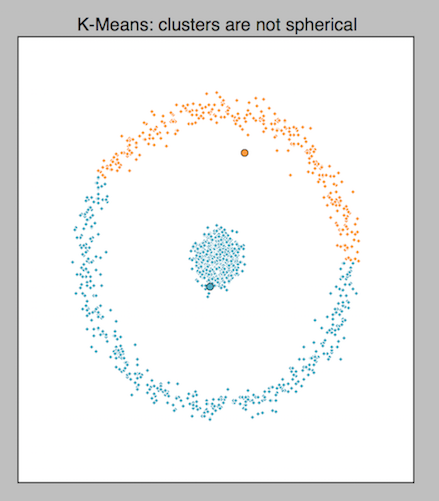
\includegraphics[width=0.7\textwidth]{k_means_not_spherical.png}
\caption{Illustration démontrant la non sphéricalité des partitions par K-Means.}
  \label{fig:k_means_not_spherical}
\end{figure}
K-Means garantit l'indépendance linéaire des centroïdes et améliore l'initialisation obtenue pour la factorisation par la suite. De plus en choisissant différents centroïdes de départ pour les algorithmes $k$ signifie, nous pouvons obtenir différents $W$ initial, de sorte que ce processus n'est pas déterministe et la sortie finale de NMF peut varier.

\subsection{Spherical K-Means}
En 2001, Dhillon et Modha ont introduit la méthode \cite{hornik2012} Spherical K-Means pour regrouper de grands ensembles de données textuelles éparses. Cette méthode a été établie en tirant parti de certains pré-traitements souvent effectués lorsque l'on travaille avec du texte dans un modèle d'espace vectoriel. Afin d'attribuer un poids égal à chacun des $n$ points d'un ensemble de données, les vecteurs de colonnes $x_{1}, x_{2}, .., x_{n}$ de la matrice de données $M\times N$ originale X sont normalisées pour être de longueur unitaire dans la norme euclidienne. L'effet de cette normalisation est de ne prendre en compte que la direction de chaque vecteur et non la longueur. Nous limitons l'ensemble de données de la matrice initiale pour qu'il soit entièrement constitué d'éléments non négatifs ce qui est une propriété naturelle de la plupart des modèles d'espace vectoriel de texte et d'image.
Une partie significative et non triviale de l'algorithme de Spherical K-Means (et respectivement K-Means) est de choisir $k$.\newline Le nombre de clusters disjoints pour partitionner les données est semblable au choix de $r$ dans une factorisation matricielle non négative, la sélection de $k$ pour Spherical K-Means reste un sujet ouvert et largement inexploré. C'est en grande partie à cause des objectifs variables que l'on peut avoir en se regroupant et de la forte dépendance d'un \textit{«rang latent»} sur le type et la structure des données. Dans des dimensions très élevées, il peut être impossible de visualiser l'ensemble de données de manière à révéler une valeur optimale pour $k$. En pratique, la borne $k << min(m,n)$ est habituellement choisie comme point de départ. Les approches pratiques pour sélectionner $k$ sont analogues à celles utilisées dans l'analyse en composantes principales où une valeur $k$ est choisie en fonction de la pente changeante de la fonction coût. Une méthode d'initialisation de ces centroïdes consiste à choisir (de façon aléatoire) chaque centroïde comme étant un vecteur de colonne différent de l'ensemble de données. Cette initialisation tente d'éviter une difficulté commune de nombreuses techniques K-Means qui se produisent lorsqu'un cluster initialisé ne contient aucun point après une itération. Pour les besoins du TER, nous avons choisi un intervalle de $k$ pour chaque ensemble de test. Une fois le nombre de clusters déterminé, l'algorithme nécessite une initialisation centroïde pour chaque nombre de classe. Il convient de noter que l'initialisation Spherical K-Means a un impact non trivial sur le schéma de cluster résultant car Spherical K-Means (comme d'autres méthodes de descente du gradient \cite{Lin2007}) sont susceptibles d'être piégés dans les maxima locaux lors de la recherche du vrai maximum global de la fonction coût donnée.


\subsection{Double décomposition en valeurs singulières non négative}
Les avantages de la SVD (Singular Value Decomposition) comprennent une propriété d'optimalité avec le fait que la SVD tronquée produit la meilleure approximation $k$ (en termes de distances au carré), puisque le calcul est rapide et robuste. Ensuite l'unicité de la factorisation car l'initialisation n'affecte pas les algorithmes SVD \cite{Boutsidis2007}.


\begin{figure}[H]
\centering
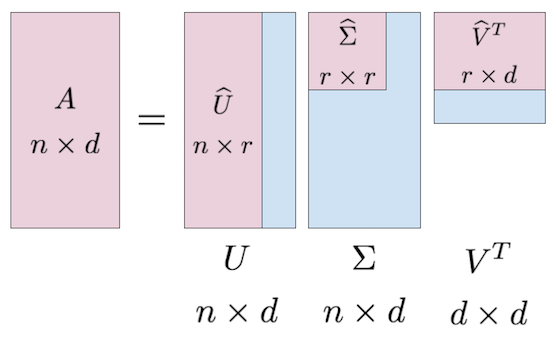
\includegraphics[width=0.8\textwidth]{svd-matrices.png}
\caption{Illustration de la SVD.}
  \label{fig:svd}
\end{figure}

Un des plus grand point faible de la NMF sont ses problèmes de convergence. Contrairement à la SVD, il n'y a pas de factorisation unique de la NMF. Les différents algorithmes de la NMF peuvent converger vers différents minima locaux (et même cette convergence vers des minima locaux n'est pas garantie), l'initialisation de l'algorithme devient critique. En pratique, la connaissance du domaine d'application peut aider à guider les choix d'initialisation.
La solution au problème sans contraintes de positivité obtenues à travers la SVD, en général ne résout pas le problème NMF, car il peut y avoir des éléments négatifs dans les matrices $W$, $H$, mais si nous mettons les éléments négatifs à zéro, ou nous effectuons un autre processus pour en faire des matrices non négatives, nous pouvons utiliser la solution SVD comme point de départ pour les algorithmes itératifs, malgré l'initialisation aléatoire de $W$ et $H$. La décomposition de valeur singulière double non négative ($NNDSVD$) tente d'ajuster la SVD d'une manière légèrement différente en produisant directement une décomposition non négative. Les variables $W$ et $H$ sont toutes deux positives, mais elles sont généralement éparses, elles sont donc modifiées en ajoutant $\epsilon$ plus petit que la moyenne des éléments aux entrées nulles. Dans le cas symétrique, cette méthode peut être ajustée pour obtenir $W = H$, et elle gagne en coût de calcul, puisque la SVD peut être remplacée par un processus de diagonalisation. Cette méthode d'initialisation n'a pas de partie aléatoire, donc un algorithme NMF ne produira qu'un seul minimum local. 

\subsection{Analyse en Composantes Principales}
Dans cette section, nous parlerons de l'ACP (Analyse en Composantes Principales). L'analyse en composantes principales est une méthode statistiques multivariée initié par K. Pearson en 1901. L'un des problèmes les plus connus dans l'exploration de données est la reconnaissance de formes, à savoir le problème de trouver des caractéristiques similaires dans différents objets. Les domaines de Text Mining et Image Processing nécessitent des méthodes pour résoudre ces problèmes afin de catégoriser les données, où pour trouver des fonctionnalités communes simples qui nous permettent de décrire les objets de manière compressée. L'un des principaux outils utilisés de nos jours pour la compression et l'identification des caractéristiques communes est l'ACP, obtenue à partir de la décomposition des valeurs singulières des données. En effet, étant donné un ensemble d'objets (images, documents, signaux, etc.), identifiés par des vecteurs réels empilés comme des colonnes de la matrice, l'analyse trouve la meilleure approximation d'un rang inférieur des données originales, et les stocke dans un espace d'ordre de grandeurs plus petites que l'entrée. Nous pouvons utiliser la SVD pour trouver les $k$ caractéristiques les plus importantes qui sont communes à tous les objets d'entrées.

\begin{figure}[H]
\centering
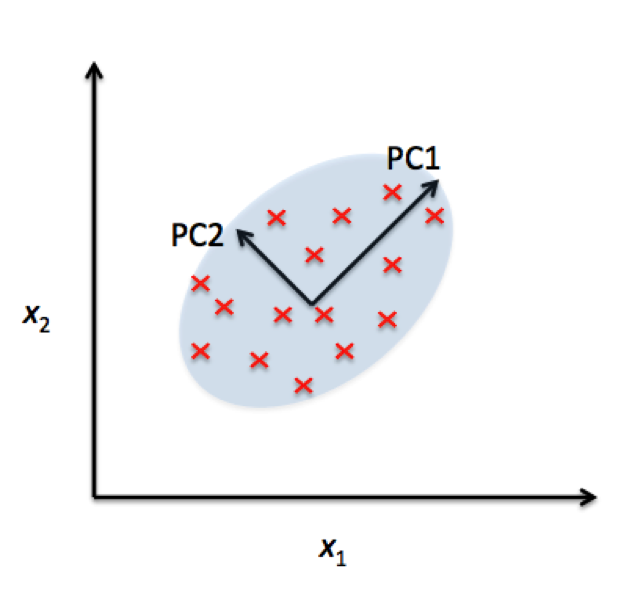
\includegraphics[width=0.6\textwidth]{pca.png}
\caption{Illustration de l'ACP.}
  \label{fig:k_means_not_spherical}
\end{figure}

La SVD nous donne la meilleure approximation $k$ de $A$ en norme $L_2$ et Frobenius, (et en général dans toute norme unitairement équivalente) et elle est relativement facile à calculer, donc largement utilisé dans beaucoup d'applications. Une particularité de l'ACP est qu'elle produit des entrées négatives dans les entités et les coefficients, même lorsque $A$ est non négatif.\newline Récemment, de nombreuses applications ont introduit la requête non négative dans leur algorithme \cite{nadif} de reconnaissance de formes afin d'obtenir l'interprétabilité de la sortie. Dans ce contexte, on peut l'utiliser dans le cadre de la NMF car sa décomposition préserve la positivité des données rendant les résultats lisibles.

\subsection{Analyse en composantes Indépendantes}
L'analyse indépendante des composants est similaire à l'ACP puisqu'elle fait également tourner une matrice dans un nouvel ensemble de coordonnées. Cependant, contrairement à l'ACP, l'objectif de l'ICA est de réaliser ensemble d'échantillons de données de sorte qu'ils soient statistiquement indépendants les uns des autres. Étant donné la matrice $X$ dont les colonnes sont des échantillons de données individuels, l'ICA tente de déterminer les matrices $A$ et $Y$ telles que les colonnes de $Y$ soient statistiquement indépendantes:

\begin{equation}
X = AY
\end{equation}

En outre, l'ICA calcule l'inverse de $A$, l'appelant $W$, de telle sorte que:

\begin{equation}
Y = WX
\end{equation}

$W$ et $A$ sont respectivement appelés matrices non mélangées et matrice de mélange parce que les observations $X$ sont considérées comme des mélanges de sources statistiquement indépendantes $Y$. L'indépendance statistique est ici définie par les densités de probabilité des échantillons. Considérons deux variables aléatoires $y_1$ et $y_2$ avec des densités de probabilité $p_1(y_1)$ et $p_2(y_2)$. Si la densité de probabilité conjointe $p(y_1, y_2)$ peut être écrite comme le produit des fonctions de densité de probabilité individuelles, alors les variables sont dites indépendantes.
Dans le cas de l'analyse d'images, l'ICA ne peut pas être appliqué directement. Le but n'est pas de déterminer les composantes dont les formes sont indépendantes les unes des autres, mais plutôt de déterminer les composantes dont les contributions relatives, sont indépendantes les unes des autres. En d'autres termes, les changements dans la contribution d'une composante devraient fournir le moins d'informations possible sur les changements dans les contributions des autres composantes. Une bonne première étape consiste alors à trouver les composantes principales des caractéristiques via l'ACP.

\begin{equation}
X = UAY
\end{equation}

Maintenant, les colonnes du produit $UA$ contiennent les composantes indépendantes qui, lorsqu'elles sont mélangées par $Y$, produisent les caractéristiques observés contenus dans les colonnes de $X$. Les graphiques concernant l'ICA sont disponibles sur le dépôt Github \href{https://github.com/mbenhamd/nmf-ter/tree/master/nmf_result}{[ici]}.

\section{\'Etude comparative}
\label{comparative}
\subsection{Estimation du rang de la NMF}

Le rang de factorisation est un paramètre très important de la NMF. Tout comme pour le nombre de cluster de K-means et Spherical K-Means. Il peut s'avérer difficile de déterminer le bon nombre de cluster. La façon la plus courante pour déterminer le nombre de cluster $k$ est d'essayer plusieurs valeurs de $k$, calculer plusieurs mesures de qualités et choisir la meilleure valeur de $k$ suivant ces critères. 
Ainsi, plusieurs approches ont été proposées afin de choisir la valeur de $k$ optimal : \\
 - La première approche est de choisir la première valeur de $r$ où le coefficient de \textit{cophenetic} commence à décroître. \\
 - Une deuxième approche consiste à choisir la première valeur de $r$ ou la courbe de \textit{RSS} présente un point d'inflexion. \\
 - Enfin, une troisième approche est de choisir $k$ quand le coefficient de silhouette est le plus élevé.


\subsection{\'Evaluation des donn\'ees}

La première étape a consisté à déterminer le meilleur rang pour la NMF. Pour cela, on a calculé la NMF sur un rang d'intervalle 20 à 70..

\begin{figure}[H]
\centering
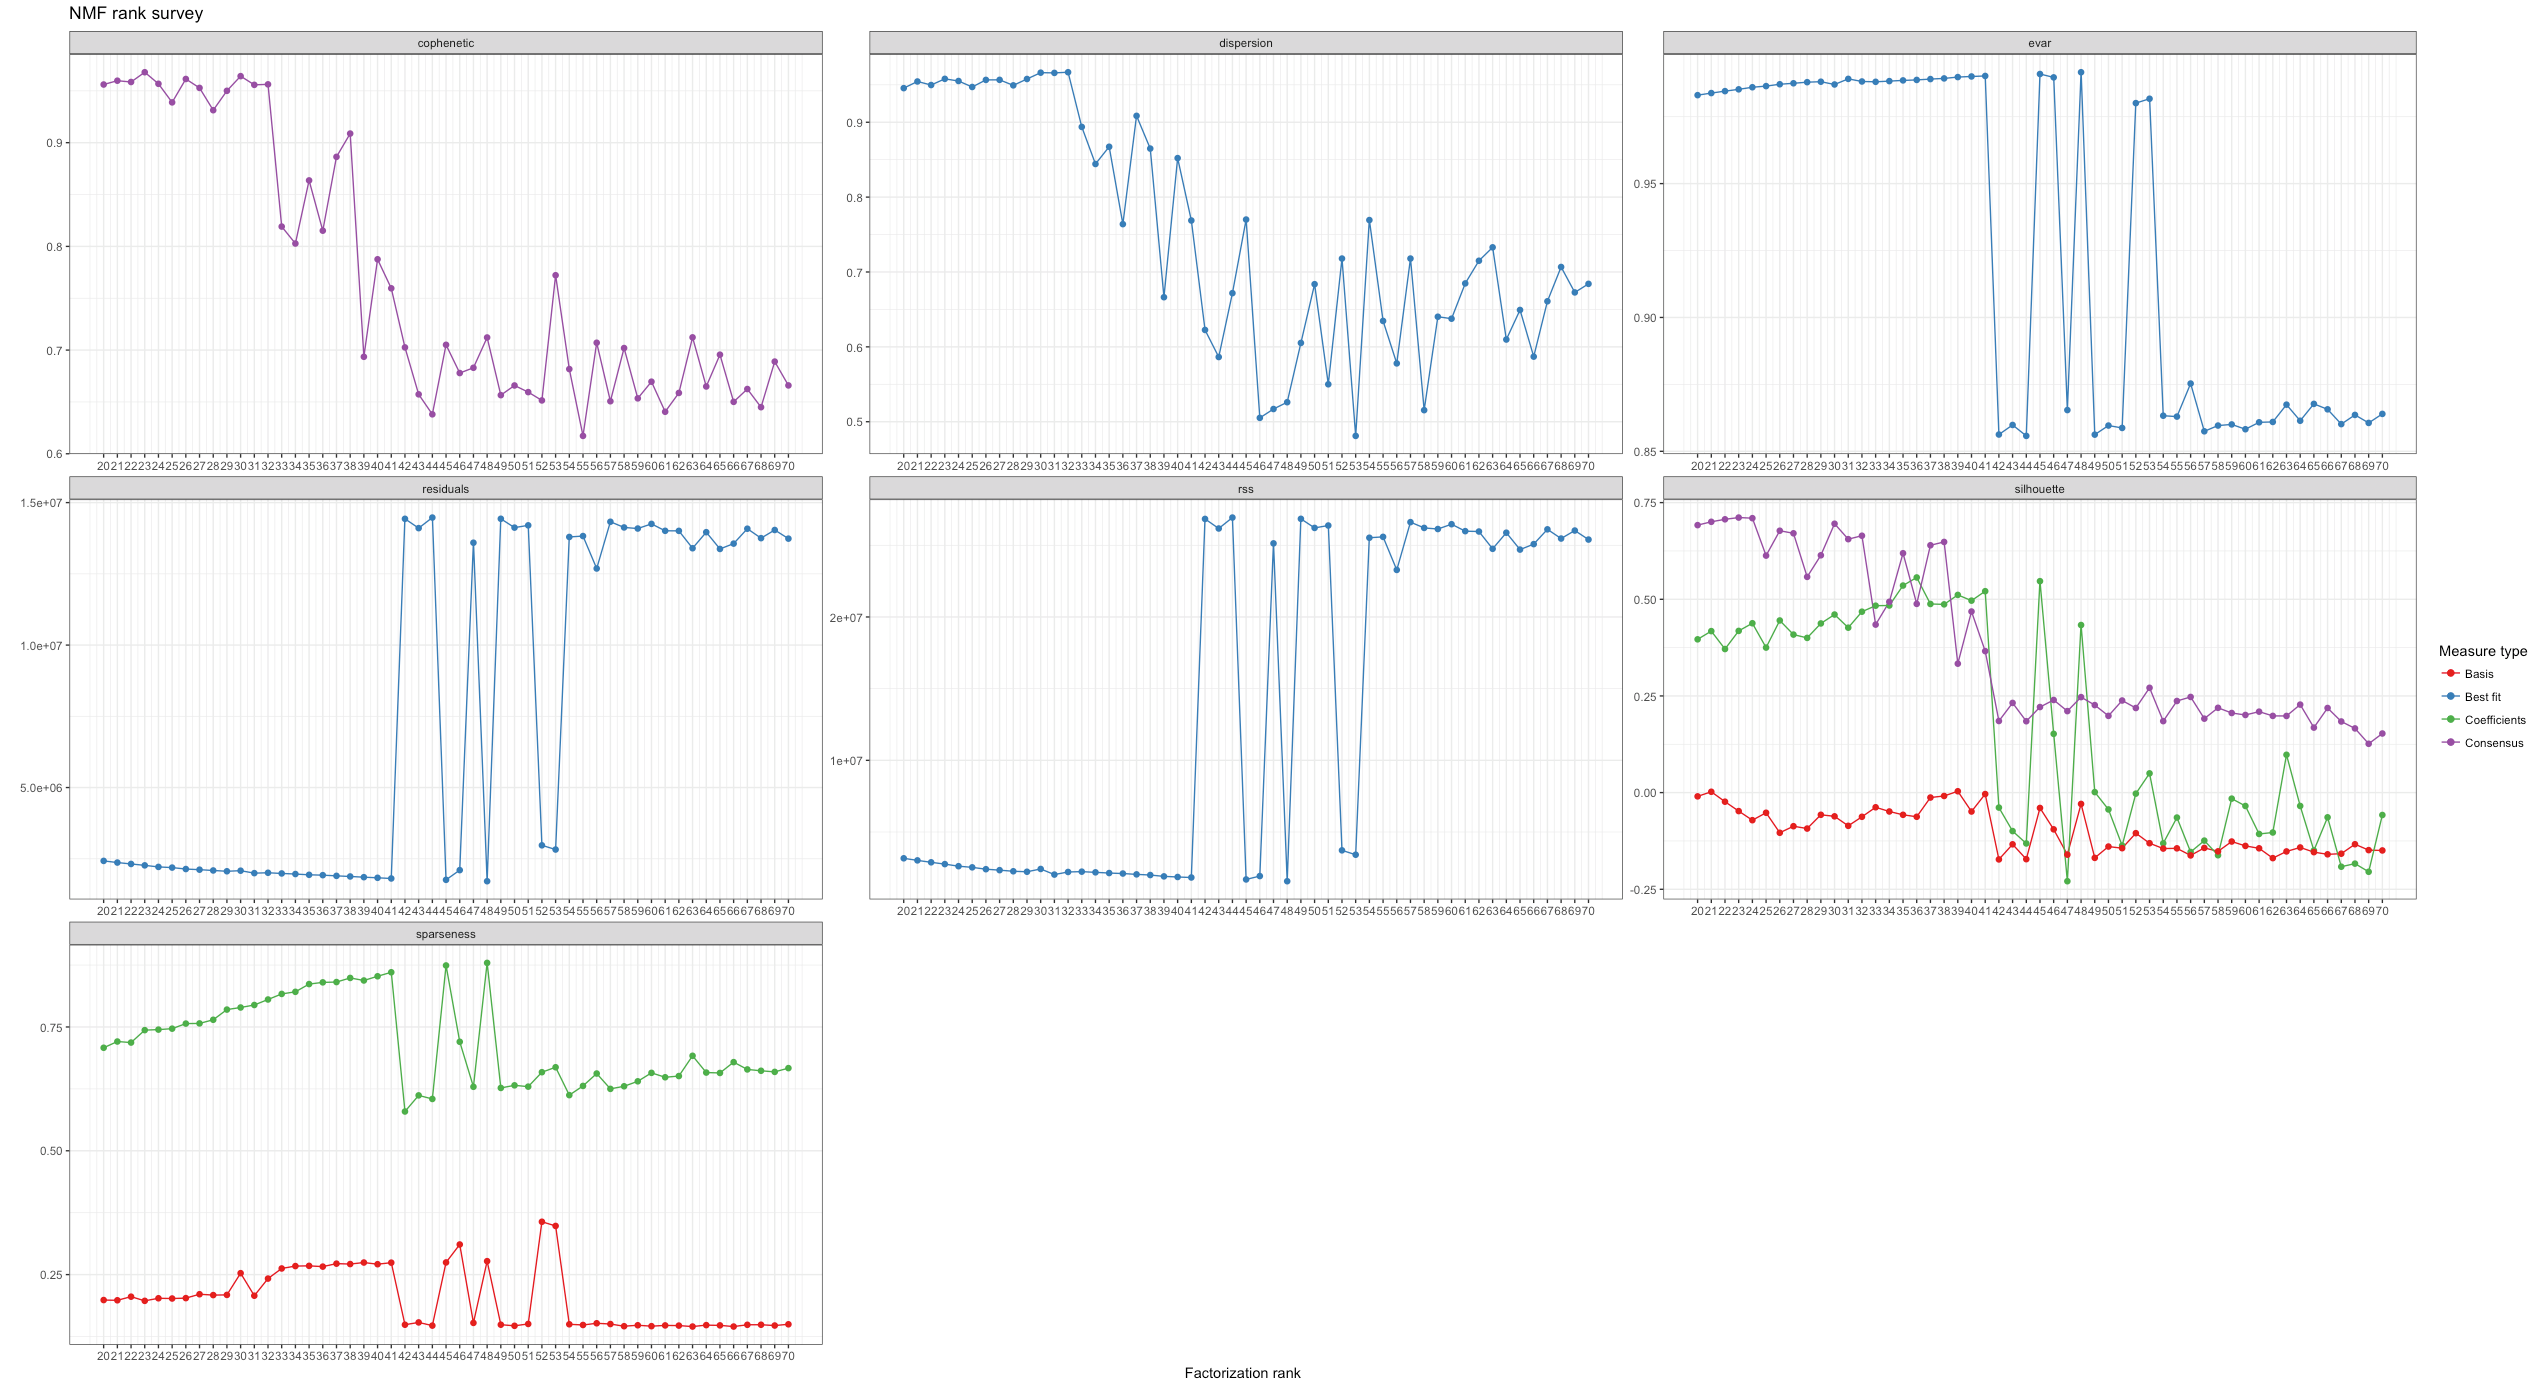
\includegraphics[width=1\textwidth]{rank20-70.png}
\caption{Récapitulatif des différents résultats obtenus pour le rang 20 à 70.}
  \label{fig:recomposition}
\end{figure}

Ainsi, ces résultats nous poussent à choisir comme rang $k = 33$. En effet, nous pouvons voir que le coefficient de cophénétique est autour de 1 avant une forte décroissance. De plus le consensus et la silhouette présentent un meilleur graphique. 

Une fois le rang déterminé, nous avons voulu tester les différentes méthodes et initialisation, le tableau ci-dessous regroupe les critères pour toutes les méthodes testées. 

\begin{figure}[H]
\centering
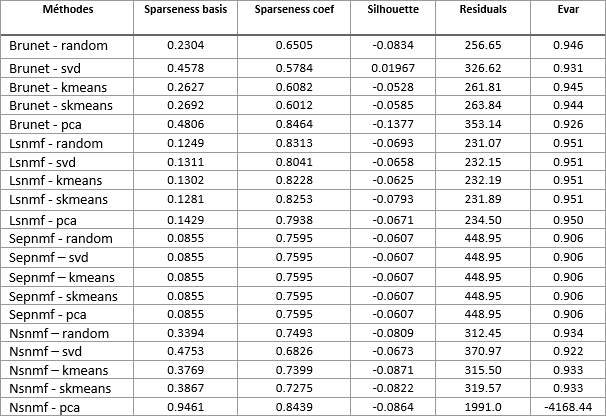
\includegraphics[width=1.0\textwidth]{tab-resultat.png}
\caption{Récapitulatif sur les différentes modèles.}
  \label{fig:tab-resultat}
\end{figure}

La colonne $Evar$ donne les valeurs obtenues pour la variance expliquée :
\begin{equation}
evar = 1 - \frac{RSS}{SST}
\end{equation}
ou $RSS$ est la somme des carrés des résidus (residual sum of squares) et où $SST$, la somme totale des carrés (total sum of squares). \\ \\
Les erreurs et les résidus sont deux mesures étroitement liées et facilement confondues de la déviation d'une valeur observée d'un élément d'un échantillon statistique à partir de sa "valeur théorique". L'erreur d'une valeur observée est l'écart de la valeur observée par rapport à la valeur vraie (inobservable) d'une quantité d'intérêt (par exemple, une moyenne de pixel ayant la même valeur dans une colonne), et le résidu d'une valeur observée est la différence entre valeur observée et la valeur estimée de la quantité d'intérêt (par exemple, une moyenne de colonne ayant les mêmes valeurs). La distinction est importante car les concepts sont parfois appelés les erreurs de régression et les résidus de régression et où ils conduisent à la notion de résiduels étudiés.

Afin de choisir la meilleure méthode, nous cherchons donc à minimiser le \textit{residuals} et maximiser la silhouette et \textit{l'Evar}. Nous pouvons voir que la méthode Lsnmf présente les meilleurs résultats pour le \textit{residuals} et \textit{l'Evar}. La méthode d'initialisation semble ne pas faire une différence, les résultats sont très similaires concernant la Lnsmf. Il est plus intéressant de choisir une initialisation aléatoire afin d'économiser du temps de calcul et de complexité.


\begin{figure}[H]
\centering
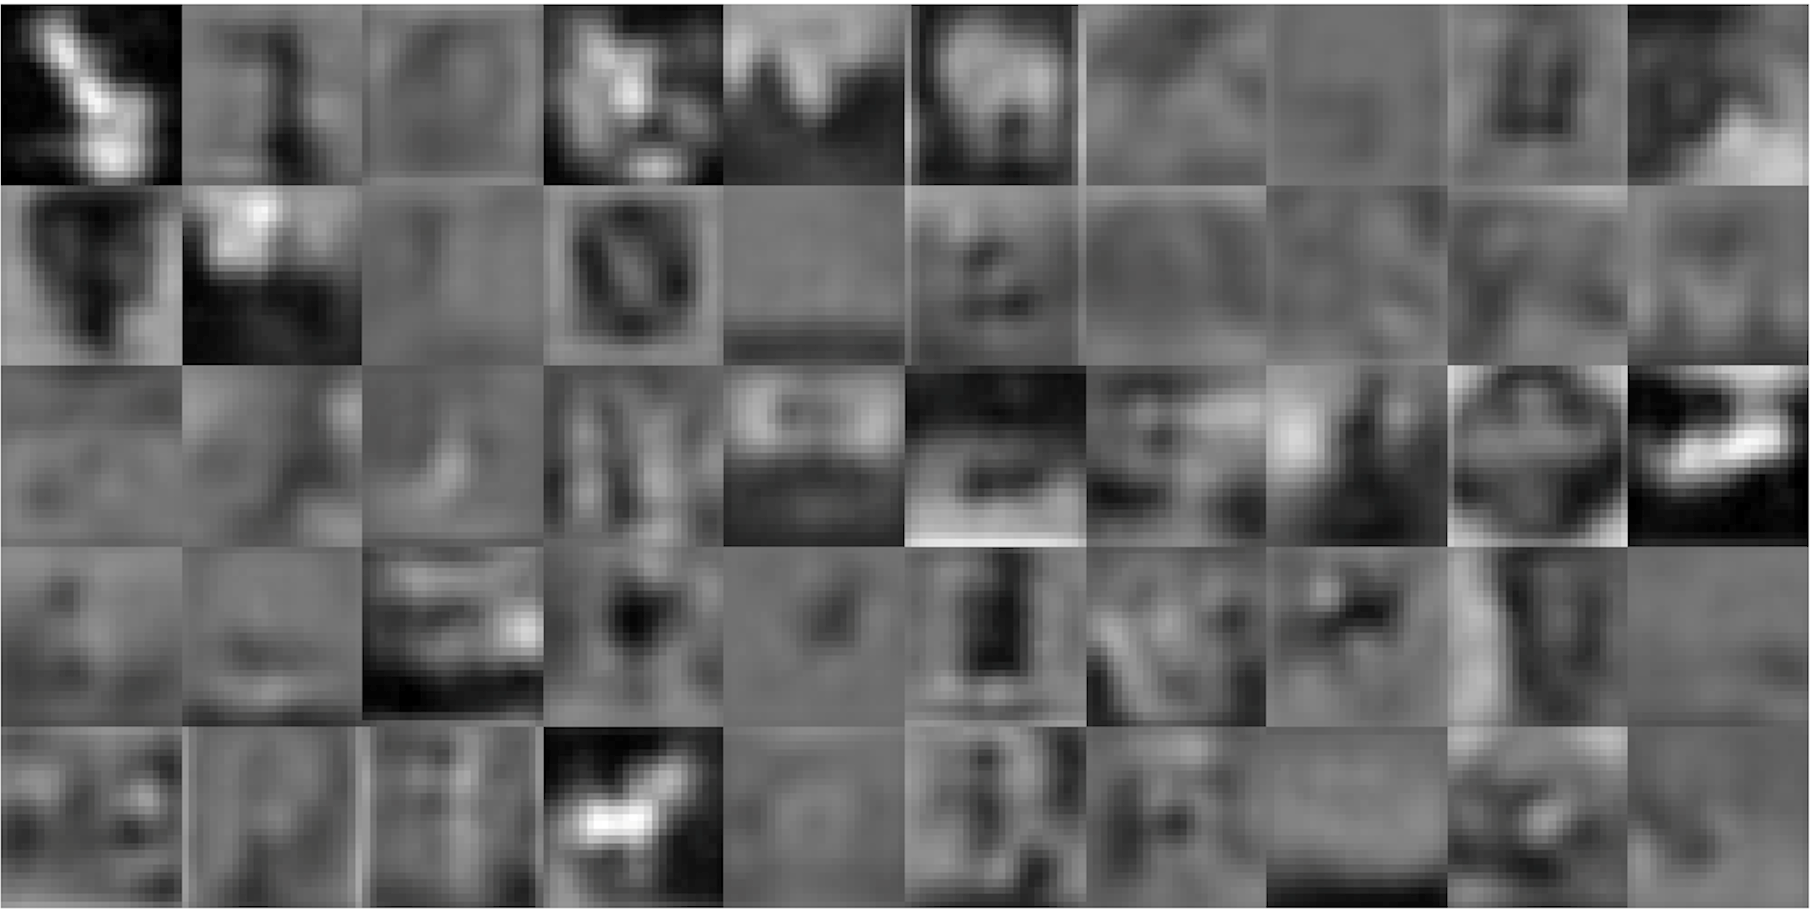
\includegraphics[width=1\textwidth]{recomposition-lsnmf-33.png}
\caption{Recomposition avec le rang 33.}
  \label{fig:recomposition}
\end{figure}

\begin{figure}[H]
\centering
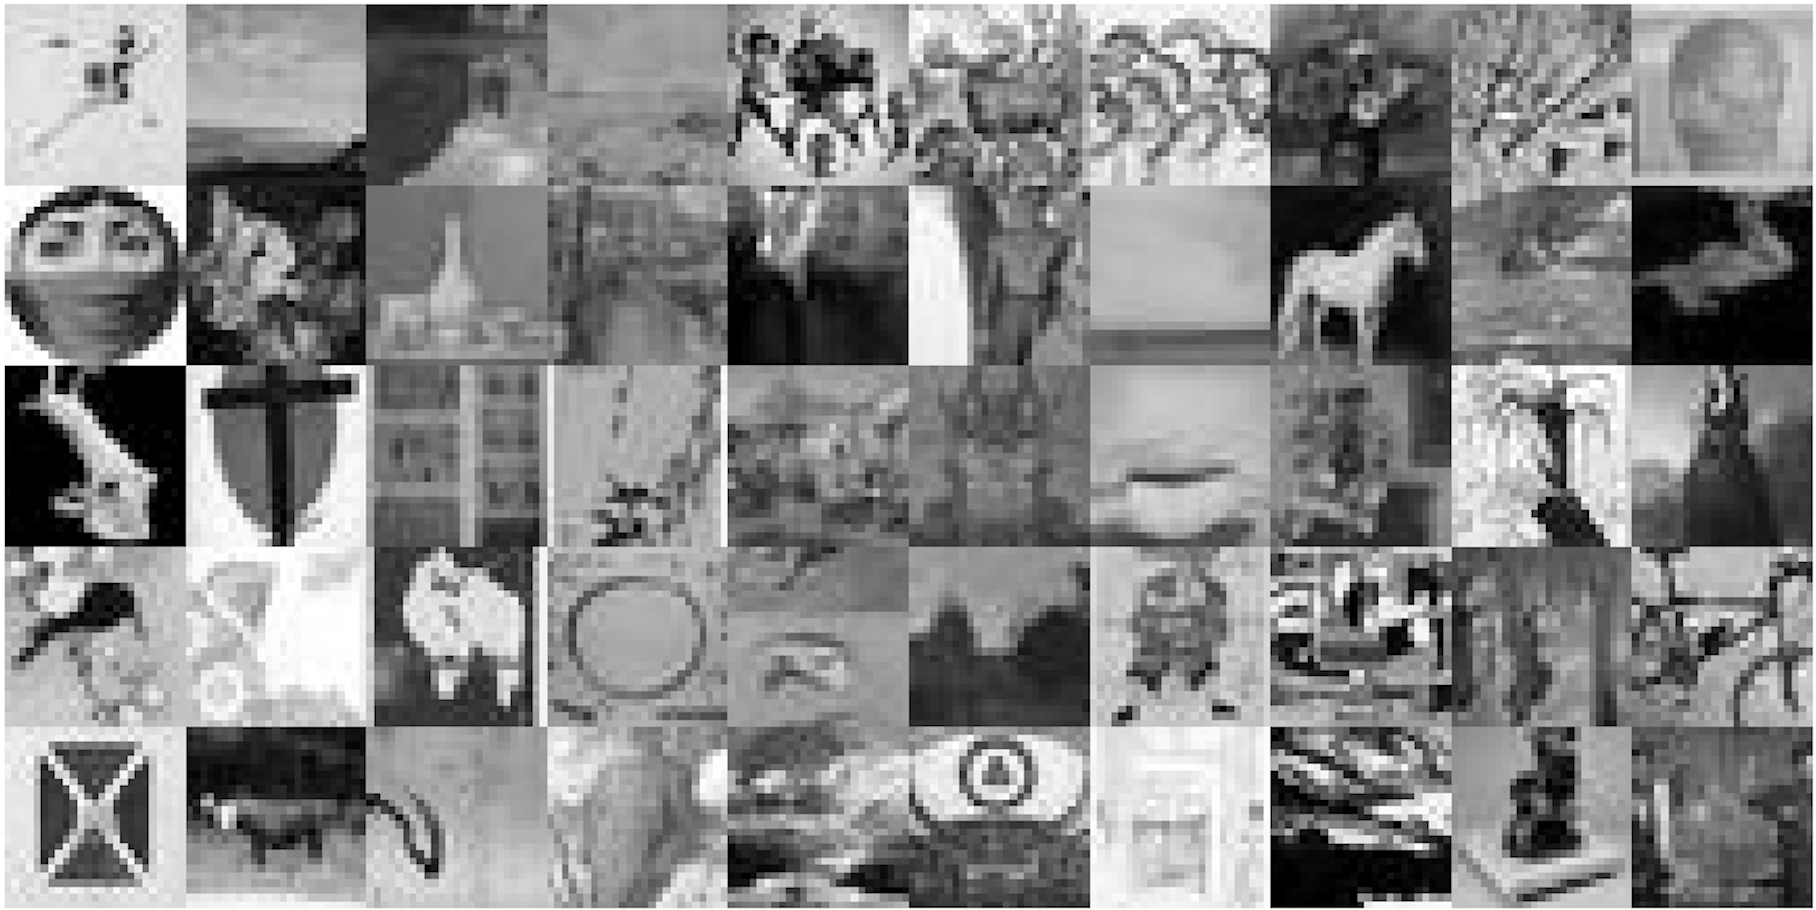
\includegraphics[width=1\textwidth]{recomposition-original-dataset.png}
\caption{Recomposition des images avec le jeu de données original.}
  \label{fig:recomposition}
\end{figure}
\newpage

\subsection{Résultats}


Après avoir déterminé le meilleur rang pour la NMF et le nombre de cluster optimal pour K-Means et Spherical K-Means, nous avons voulu comparer les partitions obtenues entre la NMF et le clustering. Pour cela nous avons calculé l'ARI et la NMI : 

\begin{figure}[H]
\centering
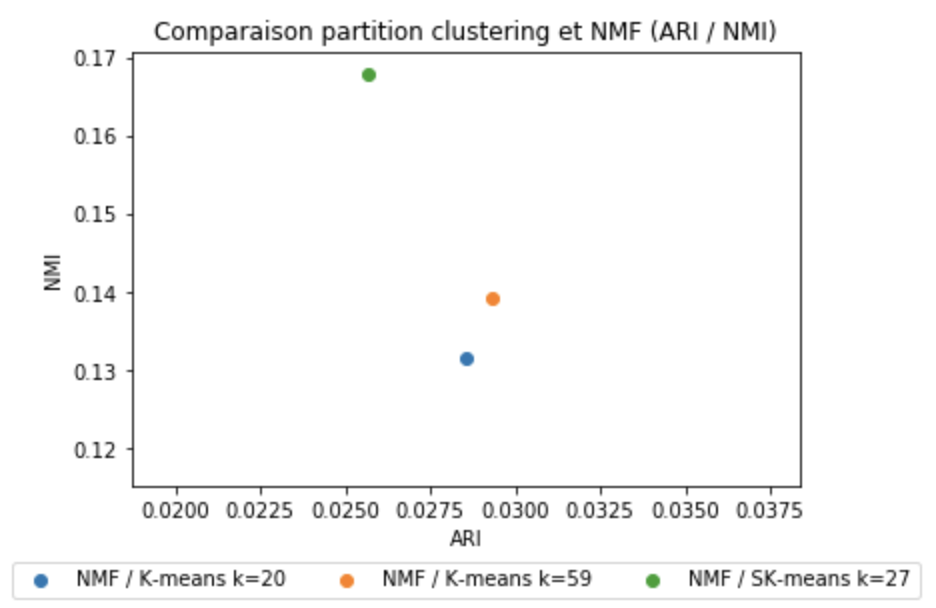
\includegraphics[width=1\textwidth]{partition.png}
\caption{Comparaison partition NMF/Clustering}
  \label{fig:recomposition}
\end{figure}

Nous pouvons voir que les résultats ARI/NMI sont très faible, ce qui signifie que les partitions obtenues avec la NMF et K-Means/Spherical K-Means sont très différentes et qu'il n'existe aucune similarité entre ces partitions. \\
Ces résultats sont cependant assez cohérent avec les résultats obtenues tout au long de ce rapport. En effet le score de silhouette des différentes initialisation de K-Means et Spherical K-Means étaient très faible aussi, ce qui peut signifier qu'il n'existe pas de bonne séparation entre les classes dans les données. Il est donc fort probable que plusieurs exécutions de K-Means nous donnent des partitions très différentes.

\newpage
\section{Conclusion}
\label{conclusion}
Pour conclure nous aborderons les cas que nous n'avons pas traités ainsi que du jeu de données en soi, le clustering est un domaine très compliqué car nous voyageons dans le flou comme on a pu le constater durant ce semestre mais nous avons appris beaucoup sur la classification automatique.
Tout d'abord, nous avons donné les différents résultats et leur explication mais cela nous a appris plusieurs choses très utiles en tant qu'étudiants en sciences des données. Même avec un pré-traitement réfléchi ou sans, finalement les résultats était mauvais ainsi qu'une multitude de combinaisons différents de la NMF (algorithmes, méthodes, initialisations) ne changeront rien au faits. Le problème vient du jeu de données qui est en soi pas adapté et correspond aux points faibles de la NMF. Les coefficients sont des nombres positifs certes mais pour chaque vecteur dans la base, la quantité d'information est généralement une petite partie que nous utilisons pour reconstruire nos points. Les lignes ayant une trop grande variété en soi ne permettent pas à la NMF de trouver un \textit{pattern}.
En particulier, il faut se rendre compte que si la NMF est beaucoup utilisée dans les sciences, son rigoureux fondement est seulement découvert depuis moins de 30 ans. Au moment où nous écrivons et il est très probable que nous n'avons pas encore trouvé le meilleur algorithme pour cela.
Ensuite, nous avons fait face à un manque de temps pour réaliser les analyses avec une matrice RGB et binaire. Il faut savoir que nous avons utilisé deux différents services de \textit{Cloud Computing} (Amazon Web Service, Google Cloud Computing), les librairies \textit{Nimfa} et \textit{NMR} pour R utilise le CPU alors que pour des calculs matriciels intense, un minimum est d'avoir recours au GPU afin de réduire drastiquement le temps de calcul. Toutes les ressources (graphiques, scripts) du projet sont disponibles [\href{https://github.com/mbenhamd/nmf-ter}{ici}].
Finalement, le jeu de données ayant était construit pour de la cross-depiction, nous pouvons affirmer que la NMF comme technique n'est pas adaptée pour ce problème là (d'autres solutions existent comme les réseaux de neurones convolutifs \cite{final} ou Deep Semi-NMF \cite{deepnmf}).

%
% ---- Bibliography ----
%
% BibTeX users should specify bibliography style 'splncs04'.
% References will then be sorted and formatted in the correct style.
%
% \bibliographystyle{splncs04}
% \bibliography{mybibliography}
%

\bibliography{ter} 
\bibliographystyle{ieeetr}

\end{document}
